%Version 2.1 April 2023
% See section 11 of the User Manual for version history
%
%%%%%%%%%%%%%%%%%%%%%%%%%%%%%%%%%%%%%%%%%%%%%%%%%%%%%%%%%%%%%%%%%%%%%%
%%                                                                 %%
%% Please do not use \input{...} to include other tex files.       %%
%% Submit your LaTeX manuscript as one .tex document.              %%
%%                                                                 %%
%% All additional figures and files should be attached             %%
%% separately and not embedded in the \TeX\ document itself.       %%
%%                                                                 %%
%%%%%%%%%%%%%%%%%%%%%%%%%%%%%%%%%%%%%%%%%%%%%%%%%%%%%%%%%%%%%%%%%%%%%

\documentclass[sn-basic,pdflatex]{sn-jnl}

%%%% Standard Packages
%%<additional latex packages if required can be included here>

\usepackage{graphicx}%
\usepackage{multirow}%
\usepackage{amsmath,amssymb,amsfonts}%
\usepackage{amsthm}%
\usepackage{mathrsfs}%
\usepackage[title]{appendix}%
\usepackage{xcolor}%
\usepackage{textcomp}%
\usepackage{manyfoot}%
\usepackage{booktabs}%
\usepackage{algorithm}%
\usepackage{algorithmicx}%
\usepackage{algpseudocode}%
\usepackage{listings}%
%%%%

%%%%%=============================================================================%%%%
%%%%  Remarks: This template is provided to aid authors with the preparation
%%%%  of original research articles intended for submission to journals published
%%%%  by Springer Nature. The guidance has been prepared in partnership with
%%%%  production teams to conform to Springer Nature technical requirements.
%%%%  Editorial and presentation requirements differ among journal portfolios and
%%%%  research disciplines. You may find sections in this template are irrelevant
%%%%  to your work and are empowered to omit any such section if allowed by the
%%%%  journal you intend to submit to. The submission guidelines and policies
%%%%  of the journal take precedence. A detailed User Manual is available in the
%%%%  template package for technical guidance.
%%%%%=============================================================================%%%%

%% Per the spinger doc, new theorem styles can be included using built in style, 
%% but it seems the don't work so commented below
%\theoremstyle{thmstyleone}%
\newtheorem{theorem}{Theorem}%  meant for continuous numbers
%%\newtheorem{theorem}{Theorem}[section]% meant for sectionwise numbers
%% optional argument [theorem] produces theorem numbering sequence instead of independent numbers for Proposition
\newtheorem{proposition}[theorem]{Proposition}%
%%\newtheorem{proposition}{Proposition}% to get separate numbers for theorem and proposition etc.

%% \theoremstyle{thmstyletwo}%
\theoremstyle{remark}
\newtheorem{example}{Example}%
\newtheorem{remark}{Remark}%

%% \theoremstyle{thmstylethree}%
\theoremstyle{definition}
\newtheorem{definition}{Definition}%



\raggedbottom




% tightlist command for lists without linebreak
\providecommand{\tightlist}{%
  \setlength{\itemsep}{0pt}\setlength{\parskip}{0pt}}





\begin{document}


\title[]{\textbf{A Predictive Modeling of Tracheostomy Readmissions}}

%%=============================================================%%
%% Prefix	-> \pfx{Dr}
%% GivenName	-> \fnm{Joergen W.}
%% Particle	-> \spfx{van der} -> surname prefix
%% FamilyName	-> \sur{Ploeg}
%% Suffix	-> \sfx{IV}
%% NatureName	-> \tanm{Poet Laureate} -> Title after name
%% Degrees	-> \dgr{MSc, PhD}
%% \author*[1,2]{\pfx{Dr} \fnm{Joergen W.} \spfx{van der} \sur{Ploeg} \sfx{IV} \tanm{Poet Laureate}
%%                 \dgr{MSc, PhD}}\email{iauthor@gmail.com}
%%=============================================================%%

\author[]{\fnm{Aabha} \sur{Latkar} \dgr{BA}}

\author[]{\fnm{Febriany} \sur{Lete} \dgr{SST}}

\author[]{\fnm{Maysen} \sur{Pagán} \dgr{BA}}



  \affil[]{\orgdiv{Master of Science in Statistical
Practice}, \orgname{Boston University}}

\abstract{Hospital readmissions following the completion of a procedure
poses significant challenges for both patients and hospitals. Being
readmitted could increase the risk of complications for patients and
introduce states of distress. For hospitals, readmissions present a
strain on resources and their reputation. This project aims to develop a
model that can predict whether a patient will be readmitted within 30
days of being discharged. After thorough data preprocessing and feature
extraction, two models were trained on patient data from 2018 and tested
on patient data from 2019 to determine predictive performance: a support
vector machine (SVM) and a random forest (RF). Using Matthew's
Correlation Coefficient to compare models, the RF model had the best
performance with a coefficient of HERE while the SVM had a coefficient
of HERE.}

\keywords{}



\maketitle

\hypertarget{sec1}{%
\section{Introduction}\label{sec1}}

In the medical field of Otolaryngology, preventing hospital readmissions
following procedures such as tracheostomies, total laryngectomies, or
mastoidectomies is significant both medically for patients as well as
financially for healthcare institutions. Medically, avoiding
readmissions can benefit patients' well-being as it reduces the possible
distress and suffering experienced from complications from new or
returning medical conditions. Financially, preventing readmissions is
crucial for hospitals who are paid by capitation. Capitation is a
payment system that pays hospitals a fixed amount per patient for a
prescribed period, therefore incentivizing hospitals to conduct less
procedures and treat patients as efficiently as possible. As a result,
hospitals paid by capitation incur the costs that are associated with
providing care to patients who are readmitted. Knowing if a patient
might be at higher risk of a readmission would allow doctors to increase
the effectiveness of their initial interventions and promote a smoother
recovery process while maintaining their reputation and quality of care.
Therefore, developing predictive models that can predict whether a
patient will be readmitted is essential for ensuring the efficiency of
healthcare. \newline \newline This project aims to build a model that
predicts if a patient who underwent a tracheostomy procedure is going to
be readmitted within 30 days of being discharged from the hospital. For
those patients who are readmitted within 30 days, this project also
analyzes the number of days until they will be readmitted as well as the
most common diagnoses that the patients will be readmitted with. The
following analysis for this project was conducted on a sample of 3
million observations from the original data.

\hypertarget{sec2}{%
\section{Data Preprocessing}\label{sec2}}

The data for this project was provided to us from the Healthcare Cost
and Utilization Project (HCUP) Nationwide Readmissions Database (NRD).
This database provides information on admissions and discharges for
patients with and without repeat hospital visits within a given year. To
address the research questions of this project, we used data from the
years of 2018 and 2019, each of which had three data sets. For each
year, there was a \texttt{core} data set which contained main
information such as the age and sex of the patient as well as the
diagnoses and procedures the patient received for this given admission.
The \texttt{severity} data set provides information on the severity of
the condition for a given admission and the \texttt{hospital} data set
contains characteristics of the hospital the patient was admitted to
such as bed size.

\hypertarget{empty-diagnoses-and-procedures}{%
\subsection{Empty Diagnoses and
Procedures}\label{empty-diagnoses-and-procedures}}

The \texttt{core} data set contains 40 ICD-10-CM diagnosis code columns
representing 40 possible diagnoses a patient could receive at one
admission. Similarly, the data includes 25 ICD-10-PCS procedure code
columns representing 25 possible procedures a patient could receive at
one admission. One patient may not have 40 total diagnoses or 25 total
procedures and as a result, many of the cells in these columns are
empty. The first step in preparing the data for analysis was replacing
these empty cells with \texttt{NA}s which will make future filtering and
one-hot-encoding steps easier.

\hypertarget{creating-binary-readmitted-response-column}{%
\subsection{Creating Binary Readmitted Response
Column}\label{creating-binary-readmitted-response-column}}

The focus of this project is predicting readmissions for tracheostomy
procedures. Therefore, our next step was to filter the \texttt{core}
data set to include only those patients who received a tracheostomy
during their admission. The ICD-10-PCS codes for tracheostomies all
begin with ``0B11'' with other numbers and letters following for
different tracheostomy approaches such as an open approach or
percutaneous approach. We applied the filter function to the 25
procedure columns to obtain all patients who had an ICD-10-PCS code that
began with ``0B11'' in any one of the 25 possible columns. Extracting
the unique IDs or Visit Links from this filtered set and filtering
\texttt{core} to get patients only with those Visit Links allowed us to
create a new data frame that contained all patients who were admitted
for a tracheostomy and all other admissions by that patient. A binary
column was then added to this new data frame which was a 1 if the
patient received a tracheostomy at the corresponding visit and 0
otherwise. For those tracheostomy admissions, we added the length of
stay (LOS) variable to the days to event variable which gives us a
sequence of numbers representing the ``date'' the patient was
discharged. This data frame contains all patient admissions both before
and after they received the tracheostomy. As a result, for each patient,
we then filtered the data frame again to include only the tracheostomy
admission and all admissions that occurred after that visit. \newline
\newline This new data frame now allows us to create our binary response
variable that is 1 if the patient was readmitted to a hospital within 30
days of being discharged from a tracheostomy procedure. If a patient had
no admissions following their tracheostomy admission, the readmitted
response variable was 0. If subtracting the days to event value of the
next admission after the tracheostomy from the days to event value of
the tracheostomy admission results in a value less than or equal to 30,
the readmitted response variable was 1. If the difference of the two
days to event values was greater than 30, the readmitted response
variable was 0. \newline \newline We then removed all rows that
represented hospital admissions after the tracheostomy to obtain a data
frame where each row represented a unique patient's tracheostomy
admission along with the binary response variable indicating if they
were readmitted within 30 days of the procedure.

\hypertarget{right-censoring}{%
\subsection{Right Censoring}\label{right-censoring}}

Right censored data is used to describe data where subjects leave the
study before an event occurring or the study ends before the event has
occurred. In the context of this project, right censoring can occur if a
patient received a tracheostomy in December of one year and was
readmitted in January of the following year. The data from the NRD is
constructed in such a way that it is difficult to identify patients. The
patient IDs or Visit Links change from one year to the next for the same
patient. As a result, if a patient were to receive a tracheostomy in
December of 2018, we would be unable to determine and therefore predict
if the patient was readmitted within 30 days since it is unknown if they
were readmitted in January of 2019. To solve this issue, we make our
window of inclusion for patients between January and November of a given
year by filtering out those patients who were admitted for a
tracheostomy in December.

\hypertarget{one-hot-encoding}{%
\subsection{One-Hot-Encoding}\label{one-hot-encoding}}

When creating the predictive model for readmissions, we wish to conduct
comorbidity analysis which will allow us to include the presence of
certain diagnoses as predictor variables. For that reason, we will need
to one-hot-encode all ICD-10-CM diagnosis codes. For each unique
diagnosis code in the 40 diagnosis columns, we added a column for that
code which equaled 1 if the patient received the diagnosis on their
tracheostomy admission and equaled 0 otherwise.

\hypertarget{joining-data-sets}{%
\subsection{Joining Data Sets}\label{joining-data-sets}}

The last step in preparing the data for modeling and analysis was to
join the three data sets. Each data set had a NRD record identifier
variable which gave a unique code to each hospital admission. Therefore,
to our cleaned \texttt{core} data set, we joined the \texttt{severity}
and \texttt{hospital} data sets by the record identifier.

\hypertarget{sec3}{%
\section{Exploratory Data Analysis}\label{sec3}}

\hypertarget{sec4}{%
\section{Methods and Analysis}\label{sec4}}

\hypertarget{predictive-model}{%
\subsection{Predictive Model}\label{predictive-model}}

\hypertarget{days-to-readmission}{%
\subsection{Days to Readmission}\label{days-to-readmission}}

Another objective of this project was to explore the number of days
until patients were readmitted for those who were readmitted within 30
days. Figure~\ref{fig:daysto} plots the counts of days to readmission
comparing males and females. \newline

\begin{figure}[H]

{\centering 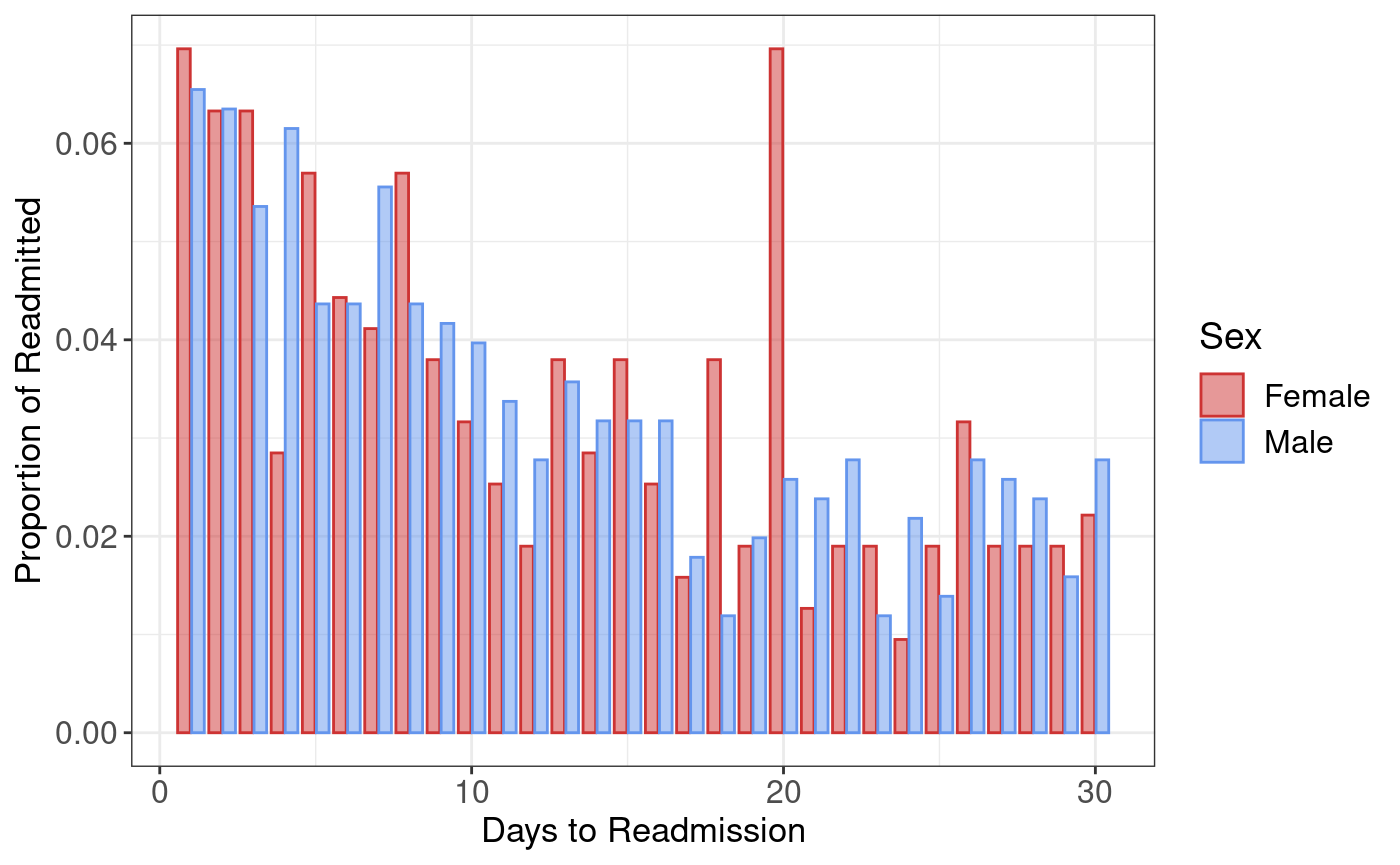
\includegraphics[width=1\linewidth]{figures/daysto} 

}

\caption{Barplot of proportion of males and proportion of females who were readmitted to a hospital after a specific number of days following discharge.}\label{fig:daysto}
\end{figure}

From this figure, we can see that most readmitted patients return to the
hospital within 10 days of being discharged from the tracheostomy. It is
interesting to note that while the largest proportion of males are
readmitted after 1 day, there is an equal proportion of females who are
readmitted after 1 day as well as after 20 days of being discharged.

\hypertarget{readmitted-diagnoses}{%
\subsection{Readmitted Diagnoses}\label{readmitted-diagnoses}}

We also created a similar figure looking at the most common diagnoses
that patients were readmitted with. For those patients who were
readmitted within 30 days of their tracheostomy discharge, we calculated
the proportion of males and the proportion of females who received a
particular diagnosis code at their readmitted visit. We then plotted
these proportions and used the proportion cutoff of 0.15 to observe the
top 15 most common readmission diagnoses.\newline \newline
Figure~\ref{fig:readmit_diags} shows that the most common readmitted
diagnosis, with an equal proportion of males and females receiving it,
is I10 which represents essential (primary) hypertension. This is
followed by A419 which is sepsis, a condition in which the body responds
improperly to an infection. Similar to hypertension, an equal proportion
of males and females are readmitted with sepsis. \newline \newline The
figure also shows that there are 4 common readmission diagnoses that
females are diagnosed with but males are not. These codes are F419,
E876, F329, and N390 which represent anxiety disorder, hypokalemia,
single episode major depressive disorder, and urinary tract infection
respectively. Within these top 15 most common readmission diagnoses,
there is one code that males are diagnosed with and females are not: E43
representing unspecified severe protein-calorie malnutrition.

\hypertarget{sec5}{%
\section{Conclusion}\label{sec5}}

\bmhead{Acknowledgments}

Acknowledgments are not compulsory. Where included they should be brief.
Grant or contribution numbers may be acknowledged.

Please refer to Journal-level guidance for any specific requirements.

\begin{appendices}

\hypertarget{secA}{%
\section{}\label{secA}}

\begin{figure}[H]

{\centering 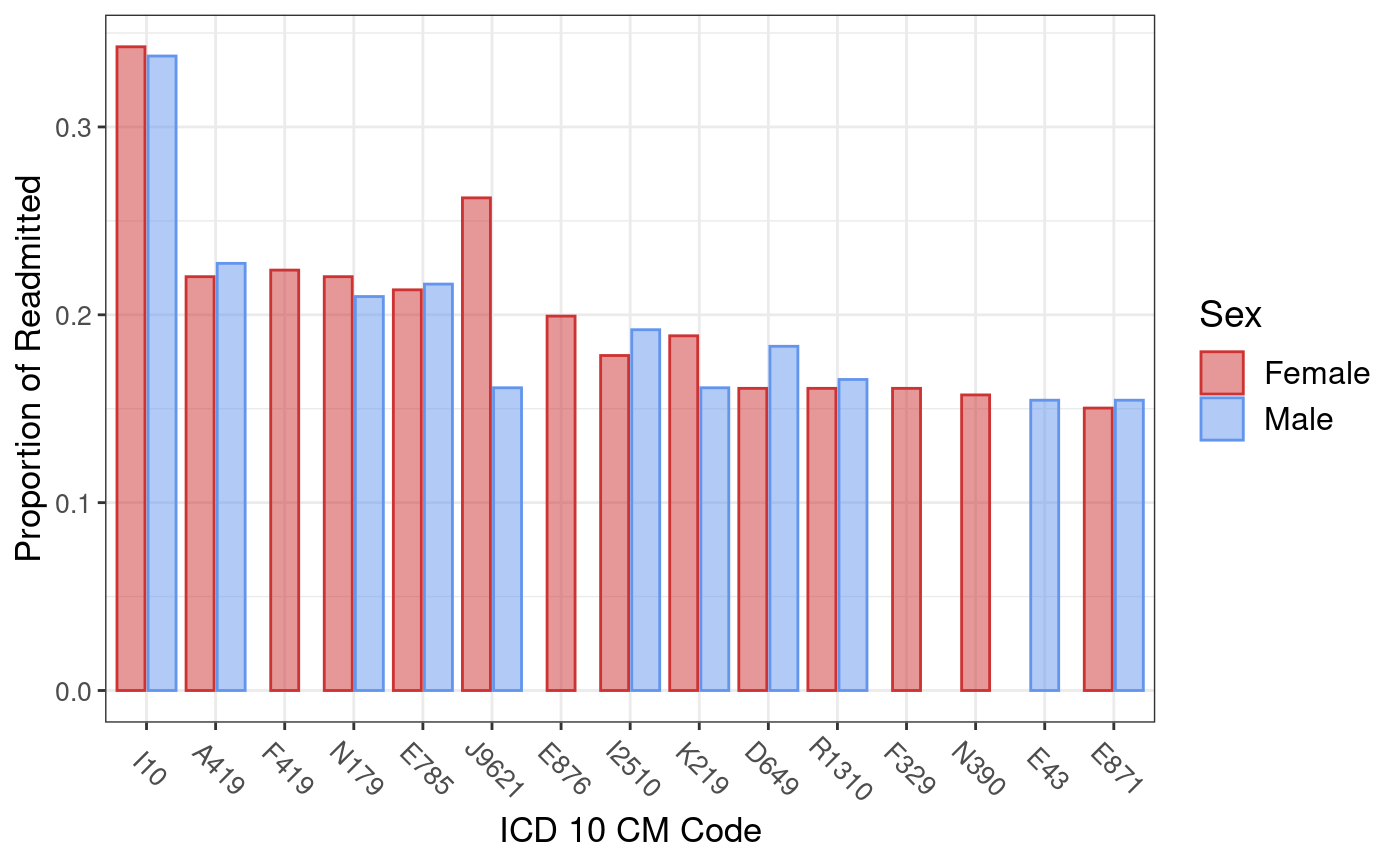
\includegraphics[width=1\linewidth]{figures/readmit_diags} 

}

\caption{Barplot of proportion of males and proportion of females who received specific diagnosis codes at their readmission visit.}\label{fig:readmit_diags}
\end{figure}

\end{appendices}

\bibliography{bibliography.bib}


\end{document}
